\documentclass[12pt,twoside, openright]{report}

\usepackage{Preambole}  % per caricare il preambolo dal file "Preambole.sty" alleggerendo il documento

% \includeonly{Head/Abstract/Abstract} %per includere solamente il capitolo che mi interessa rivedere (scrivere l'intero indirizzo)
% \includeonly{Body/Introduction/Introduction}
% \includeonly{Body/Projects/Projects}
% \includeonly{Body/Conclusions/Conclusions}
% \includeonly{Tail/Appendix/Appendix}
% per ultima compilazione controllare di aver scommentato tutto il necessario

\begin{document}
\emergencystretch 2em  % aumenta il limite per lo stretching delle parole, in modo da permettere che una parola venga mandata a capo anche se la riga rimarrebbe con le parole molto allargate (dicono sia meglio usare questo che sloppy)
% %per inserire una pagina (due facciate) vuote, Messa perchè sta bene una pagina bianca dopo la copertina (non so perchè clearpage... non funziona)
% \newpage
% \thispagestyle{empty}
% \mbox{}
% \newpage
% \thispagestyle{empty}
% \mbox{}

\includepdf{Frontespizio/Frontespizio.pdf}
\clearpage{\pagestyle{empty}\cleardoublepage}  % per aggiungere una pagina vuota (se questa è dispari ne aggiunge un'altra ancora)

\begin{titlepage}
\thispagestyle{empty}
\topmargin=6.5cm
\begin{flushright}
\large\textit{}
\end{flushright}
\newpage
\clearpage{\pagestyle{empty}\cleardoublepage}  % per aggiungere una pagina vuota (se questa è dispari ne aggiunge un'altra ancora)
\end{titlepage}

\pagenumbering{Roman}

\fancyhf{}  % cancella tutti i campi

\chapter*{Abstract \\ \small}
% \addcontentsline{toc}{chapter}{Abstract}

\lipsum[1-10]

% \clearpage{\pagestyle{plain}\cleardoublepage}  % per aggiungere una pagina vuota (se questa è dispari ne aggiunge un'altra ancora)


\clearpage{\pagestyle{plain}\cleardoublepage}  % per aggiungere una pagina vuota (se questa è dispari ne aggiunge un'altra ancora)


% \addcontentsline{toc}{chapter}{Contents}
\tableofcontents
\clearpage{\pagestyle{plain}\cleardoublepage}  % per aggiungere una pagina vuota (se questa è dispari ne aggiunge un'altra ancora)


\chapter*{List of Acronyms and Abbreviations}
\addcontentsline{toc}{chapter}{List of Acronyms and Abbreviations}
\begin{description}
    \item[AD] Alzheimer's Disease
    \item[ADR] Adverse Drug Reaction
    \item[AI] Artificial Intelligence
    \item[AMRR] Adjusted Mean Reciprocal Rank
    \item[APCC] Average Pearson Correlation Coefficient
    \item[ATC] Anatomical Therapeutic Chemical (code)
    \item[AUC-ROC] Areas Under the Receiver Operating Characteristic Curve
    \item[CAG] Cytosine-Adenosine-Guanine
    \item[CNS] Central Nervous System
    \item[CSN] Chemical Space Network
    \item[DP] Drug Projection
    \item[DT] Drug-Target
    \item[EMA]  European Medicines Agency
    \item[ER] Erdös and Rényi
    \item[FAERS] FDA Adverse Event Reporting System
    \item[FDA] Food and Drug Administration
    \item[FDR] False Discovery Rate
    \item[GBM] Glioblastoma
    \item[GML] Graph Machine Learning
    \item[GNN] Graph Neural Network
    \item[GO] Gene Ontology
    \item[HD] Huntington's Disease
    \item[HPO] Human Phenotype Ontology
    \item[IGSEA] Inverted Gene Set Enrichment Analysis
    \item[JADER] Japanese Adverse Drug Event Report
    \item[KG] Knowledge Graph
    \item[KGE] Knowledge Graph Embedding
    \item[KGEM] Knowledge Graph Embedding Model
    \item[LCWA] Local Closed-World Assumption
    \item[LP] Link Prediction
    \item[MLP] Multilayer Perceptron
    \item[MMP] Matched Molecular Pair
    \item[MRR] Mean Reciprocal Rank
    \item[MS] Multiple Sclerosis
    \item[NHGRI] National Human Genome Research Institute
    \item[NLP] Natural Language Processing
    \item[NSSA] Self-Adversarial Negative Sampling
    \item[OOV] Out-Of-Vocabulary
    \item[PMI] Pointwise Mutual Information
    \item[PPI] Protein-Protein Interaction
    \item[PPMI] Positive Pointwise Mutual Information
    \item[PRAC]Pharmacovigilance Risk Assessment Committee
    \item[PRR] Proportional Reporting Ratio
    \item[QoL] Quality of Life
    \item[QSAR] Quantitative Structure-Activity Relationship
    \item[sLCWA] Stocastic Local Closed-World Assumption
    \item[SMILES] Simplified Molecular Input Line Entry System
    \item[SRL] Statistical Relational Learning
    \item[TCGA] The Cancer Genome Atlas
    \item[TP] Target Projection
    \item[TSV] Tab-Separated Values
    \item[VAERS] Vaccine Adverse Event Reporting System
\end{description}

\clearpage{\pagestyle{plain}\cleardoublepage}  % per aggiungere una pagina vuota (se questa è dispari ne aggiunge un'altra ancora)


% \addcontentsline{toc}{chapter}{Mathematical Notations}
% \clearpage{\pagestyle{plain}\cleardoublepage}  % per aggiungere una pagina vuota (se questa è dispari ne aggiunge un'altra ancora)

\pagenumbering{arabic}

\setcounter{chapter}{-1}  % per partire numerazione capitoli da zero (e non da uno)

% ripetere formattazione header preabole sospesa per abstract

\fancyhf{}  % cancella tutti i campi
\fancyhead[LE]{\leftmark}  % a quanto pare questi comandi devono essere separati altrimenti fa casino
\fancyhead[RO]{\rightmark}  %
\fancyfoot[LE,RO]{\thepage}  %

\part{Introduction\label{part:introduction}}

% \epigraph{\textit{Everything should be made as simple as possible, but not simpler.}}{\vspace{15pt}--- Roger Sessions paraphrasing Albert Einstein\vspace{30pt}}
% % https://quoteinvestigator.com/2011/05/13/einstein-simple/
% % https://www.nature.com/articles/d41586-018-05004-4
% % It can scarcely be denied that the supreme goal of all theory is to make the irreducible basic elements as simple and as few as possible without having to surrender the adequate representation of a single datum of experience.

% Preamble
\chapter{Thesis Overview\label{ch:thesis_overview}}
    \lipsum[1]
    \hyperref[part:introduction]{Introduction}, \hyperref[part:projects]{Projects}, and \hyperref[part:conclusions]{Conclusions}.\\

\chapter{Chapter 1\label{ch:chapter 1}}
    \lipsum[1-10]

\chapter{Chapter 2\label{ch:chapter 2}}
    \lipsum[1-10]

\chapter{Aim of the Work\label{ch:aim}}
    \lipsum[1]

% \clearpage{\pagestyle{plain}\cleardoublepage} %per aggiungere una pagina vuota (se questa è dispari ne aggiunge un'altra ancora)

\part{Projects\label{part:projects}}
% \epigraph{\textit{Everything that living things do can be understood in terms of the jiggling and wiggling of atoms}}{\vspace{15pt}--- Richard Feynman, \textit{Lecture}\vspace{30pt}}

\chapter{Projects Overview}
    \lipsum[1-4]
    \clearpage{\pagestyle{empty}\cleardoublepage}  % per aggiungere una pagina vuota (se questa è dispari ne aggiunge un'altra ancora)

\chapter{Descriptive Models\label{ch:descriptive_models}}
    
    \section{Project 1\label{prj:project1}}
    \lorem[1]

\subsection*{Details}
\begin{description}
    \item[Authors] \href{http://orcid.org/0000-0002-3397-7737}{\underline{Luca Menestrina}}, \href{https://orcid.org/0000-0001-9518-5412}{Chiara Cabrelle}, \href{http://orcid.org/0000-0002-0039-0518}{Maurizio Recanatini}
    \item[Type] Research Article
    \item[Status] Published
    \item[Title] \href{https://www.nature.com/articles/s41598-021-98812-0}{COVIDrugNet: a network‑based web tool to investigate the drugs currently in clinical trial to contrast COVID‑19}
    \item[Journal] Scientific Reports
    \item[DOI] \href{http://doi.org/10.1038/s41598-021-98812-0}{10.1038/s41598-021-98812-0}
    \item[Data Availability] The full code for the collection, building and analysis of the networks is available in the GitHub repository at \url{https://github.com/LucaMenestrina/COVIDrugNet}. It is entirely written in Python. All data generated or analyzed in this study is publicly available on the GitHub repository. Furthermore, some data is easily downloadable from the web tool itself: all tables in tab-separated values (tsv) format and the networks in various formats (adjacency list, pickle, cytoscape json, graphml, gexf, edges list, multiline adjacency list, tsv, png and jpg).\\
    Supplementary data can also be accessed at the \href{https://www.nature.com/articles/s41598-021-98812-0#Sec19}{original publication}.
\end{description}
\clearpage

\section*{Title}

% \subsection{Abstract}

\subsection{Introduction}
    \lipsum[1-5]

\subsection{Results and Discussion}
    \lipsum[1-10]

\subsection{Limitations}
    \lipsum[1-2]

\subsection{Conclusions}
    \lipsum[1]

\subsection{Methods}
    \lipsum[1-8]
    \clearpage{\pagestyle{empty}\cleardoublepage}  % per aggiungere una pagina vuota (se questa è dispari ne aggiunge un'altra ancora)
    
    \section{Project 2\label{prj:project2}}
    \clearpage{\pagestyle{empty}\cleardoublepage}  % per aggiungere una pagina vuota (se questa è dispari ne aggiunge un'altra ancora)


\chapter{Predictive Models\label{ch:predictive_models}}
    
    \section{Project 3\label{prj:project3}}
    \clearpage{\pagestyle{empty}\cleardoublepage}  % per aggiungere una pagina vuota (se questa è dispari ne aggiunge un'altra ancora)

    \section{Project 4\label{prj:project4}}
    \clearpage{\pagestyle{empty}\cleardoublepage}  % per aggiungere una pagina vuota (se questa è dispari ne aggiunge un'altra ancora)


\chapter{Data Analysis\label{ch:data_analysis_models}}
    
    \section{Project 5\label{prj:project5}}
    \clearpage{\pagestyle{empty}\cleardoublepage}  % per aggiungere una pagina vuota (se questa è dispari ne aggiunge un'altra ancora)


\clearpage{\pagestyle{plain}\cleardoublepage} %per aggiungere una pagina vuota (se questa è dispari ne aggiunge un'altra ancora)


\part{Conclusions\label{part:conclusions}}
% \epigraph{\textit{Theory is when you know everything and nothing works; practice is when everything works and nobody knows why. Here we combine theory with practice: nothing works and nobody knows why.}}{\vspace{15pt}--- Albert Einstein \vspace{30pt}}

\chapter{Outcomes and Future Perspectives}
    \lipsum[1]

    % \section*{Outcomes}
    \lipsum[1-2]

    % \section*{Limitations}
    \lipsum[1-2]

    % \section*{Perspectives}
    \lipsum[1-2]

    % \section*{Conclusions}
    \lipsum[1]

% \clearpage{\pagestyle{plain}\cleardoublepage} %per aggiungere una pagina vuota (se questa è dispari ne aggiunge un'altra ancora)


\part{References}  % references al posto di bibliography (più corretto https://apastyle.apa.org/style-grammar-guidelines/references/lists-vs-bibliographies)

\begingroup

\renewcommand\bibname{}  % tolto il titolo perchè è già scritto in una pagina a parte
\phantomsection\label{ch:references}
\printbibliography[]  % Crea e stampa la bibliografia (e la aggiunge all'indice) Prende info da Bibliography.bib  % heading=bibintoc

\endgroup

% \clearpage{\pagestyle{plain}\cleardoublepage}  % per aggiungere una pagina vuota (se questa è dispari ne aggiunge un'altra ancora)

\part{Appendices}

\phantomsection
\addcontentsline{toc}{chapter}{List of Figures}
\listoffigures
\clearpage{\pagestyle{plain}\cleardoublepage}  % per aggiungere una pagina vuota (se questa è dispari ne aggiunge un'altra ancora)

\phantomsection
\addcontentsline{toc}{chapter}{List of Tables}
\listoftables
\clearpage{\pagestyle{plain}\cleardoublepage}  % per aggiungere una pagina vuota (se questa è dispari ne aggiunge un'altra ancora)

\begingroup
% \let\cleardoublepage\clearpage

\begin{appendices}
\appendix
%\VerbatimInput[fontsize=\scriptsize, baselinestretch=0.9]{Inputfiles/Filename}

\chapter{Appendix 1}
    \begin{figure}[!htb]
        \centering
        \caption[Degree Distribution]{\textbf{Degree Distribution.} The degree distributions of both the drug (a) and target (b) projections (red), compared to those of equivalent random graphs (blue). The last ones were generated with the Erdős-Rényi model\autocite{Erds1959}, keeping the same number of nodes and probability of edge creation (ratio between the actual number of edges and the maximum possible edges) of the network they are compared with.}
        \label{fig:SI_degree_distribution}
        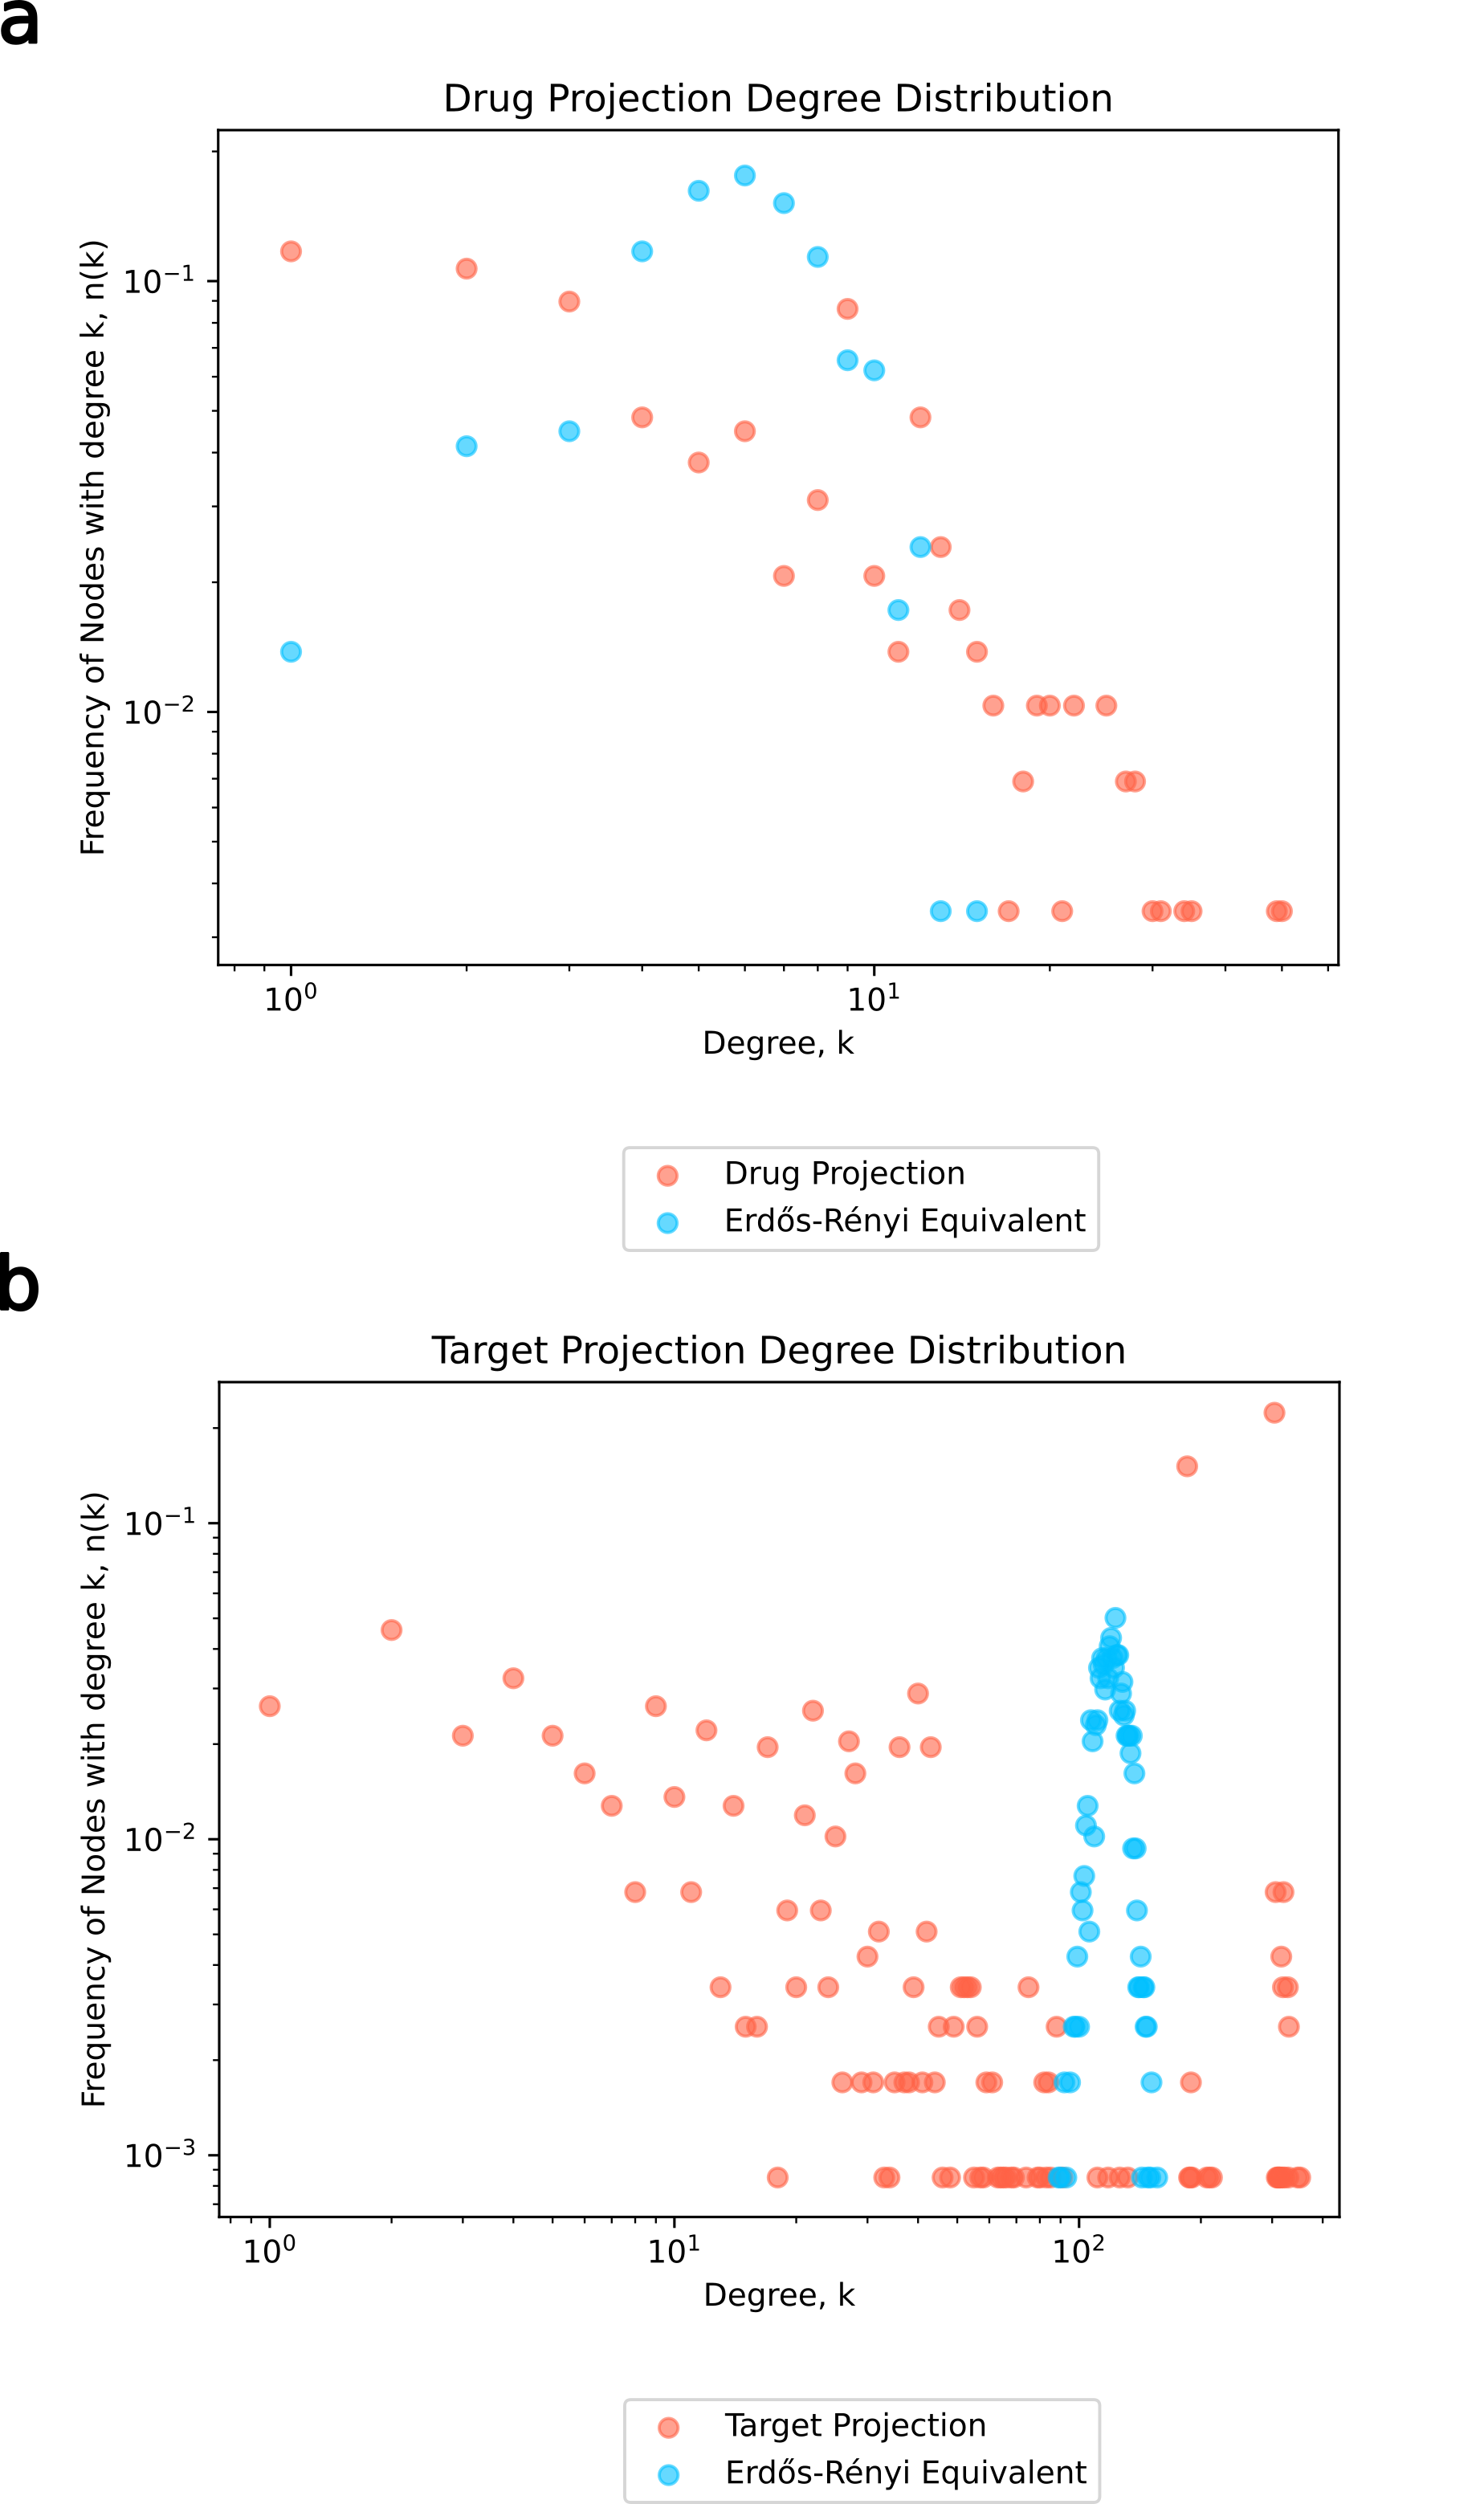
\includegraphics[width=(\textwidth/100)*80]{Images/Project1/SI/Figure_S1.png}
    \end{figure}

    \begin{table}[!htb]
        \footnotesize
        \centering
        \caption[Fittings Evaluation]{\textbf{Fittings Evaluation.} The table provides the log-likelihood and respective p-value for each function fitted on every analyzed network. For the power-law function, the Kolmogorov-Smirnov distance (D) is provided, and the fitting is considered plausible if the respective p-value is at least 0.1.}\label{tab:fittings_evaluation}
        \begin{tabular}{ccccc}
             & \multicolumn{2}{c}{\thead{Drug Projection (Entire)}} & \multicolumn{2}{c}{\thead{Drug Projection}} \\\midrule
             & D & p-value & D & p-value \\\toprule
            Power-Law & 0.07 & 2.4 $\times 10^{-1}$ & 0.05 & 3.3 $\times 10^{-1}$ \\\midrule
             & Likelihood-ratio & p-value & Likelihood-ratio & p-value \\\toprule
            Truncated Power-Law & -0.58 & 2.8 $\times 10^{-1}$ & -8.01 & 6.3 $\times 10^{-5}$ \\\midrule
            Exponential & 0.91 & 6.9 $\times 10^{-1}$ & 15.71 & 6.6 $\times 10^{-2}$ \\\midrule
            Stretched Exponential & -0.42 & 5.8 $\times 10^{-1}$ & -6.80 & 4.8 $\times 10^{-3}$ \\\midrule
            Lognormal & -0.33 & 5.9 $\times 10^{-1}$ & -5.92 & 7.1 $\times 10^{-3}$ \\\bottomrule\bottomrule
             & \multicolumn{2}{c}{\thead{Target Projection (Entire)}} & \multicolumn{2}{c}{\thead{Target Projection}} \\\midrule
             & D & p-value & D & p-value \\\toprule
            Power-Law & 0.22 & 0.0 & 0.06 & 9.5 $\times 10^{-2}$ \\\midrule
             & Likelihood-ratio & p-value & Likelihood-ratio & p-value \\\toprule
            Truncated Power-Law & -329.39 & 0.0 & -9.43 & 1.4 $\times 10^{-5}$ \\\midrule
            Exponential & -349.29 & 1.0 $\times 10^{-21}$ & -3.57 & 5.6 $\times 10^{-1}$ \\\midrule
            Stretched Exponential & -397.78 & 1.66 $\times 10^{-54}$ & -9.27 & 6.6 $\times 10^{-4}$ \\\midrule
            Lognormal & -317.17 & 1.1 $\times 10^{-51}$ & -8.86 & 1.1 $\times 10^{-3}$ \\\bottomrule
        \end{tabular}
    \end{table}

\end{appendices}
\endgroup
% \clearpage{\pagestyle{plain}\cleardoublepage}  % per aggiungere una pagina vuota (se questa è dispari ne aggiunge un'altra ancora)

\chapter*{Ringraziamenti}
\thispagestyle{empty}

\noindent
\lipsum[1-5]


% \clearpage{\pagestyle{empty}\cleardoublepage}  % per aggiungere una pagina vuota (se questa è dispari ne aggiunge un'altra ancora)
% \newpage  % per aggiungere pagina vuota
% \thispagestyle{empty}
% \vspace*{\fill}
% \clearpage{\pagestyle{empty}\cleardoublepage}  % per aggiungere una pagina vuota (se questa è dispari ne aggiunge un'altra ancora)

% %per inserire una pagina (due facciate) vuote, Messa perchè sta bene una pagina bianca subito prima della copertina (non so perchè clearpage... non funziona)
% \newpage
% \thispagestyle{empty}
% \mbox{}
% \newpage
% \thispagestyle{empty}
% \mbox{}

\listofchanges[title={ToDos, Changes...}]  % per avere un elenco di tutti i commenti e i cambiamenti fatti (quando nel preambolo metto final e non draft non compare)

\end{document}

